% Čia yra literatūros apžvalga. Šitas mokslininkas padarė taip \cite{horvath2016}.
% %
% Kitas klausimas.
%
% Toliau apžvelgsime \cite{ezhov1969} darbus.
%
% https://machinelearningmastery.com/learning-rate-for-deep-learning-neural-networks/

\subsection{Neuroniniai tinklai}
Neuroniai tinklai arba kitaip dirbtinio intelekto neuroniai tinklai yra mašininio mokymo metodai, kurie leidžia kompiuteriui mokytis iš stebimų duomenų. Neuroninių tinklų veikimo principas yra įkvėptas pagal tai kaip biologinė nervų sistema apdoroja informaciją.\cite{Sukhadeve2017}

Neuroniai tinklai dažniausiai yra naudojami išvesti prasmę iš sudėtingų netiesinių duomenų, nustatyti ir ištraukti modelius, kurie yra sunkiai pastebimi ar net išvis neįmanoma nustatyti modelio, kuris aprašytų esamus duomenis.\cite{Sukhadeve2017}



\subsection{Neuroninių tinklų neuronai}
% Neuroninių tinklų sprendžiamos problemos

Esminis neuroninio tinklo elementas yra dirbtinis neuronas. Šį neuroną sudaro pagrindiniai trys komponentai: įvesties reikšmės, svoriai, kurie jungia šias reikšmes su neuronu ir aktyvacijos funkcija. \ref{fig:perceptron1} Tai yra pats paprasčiausias neurono modelis, vadinamas Perceptronu (angl. \textit{Perceptron}).\cite{Andrew2017}

\begin{figure}[h!]
  \centering
\scalebox{0.2}{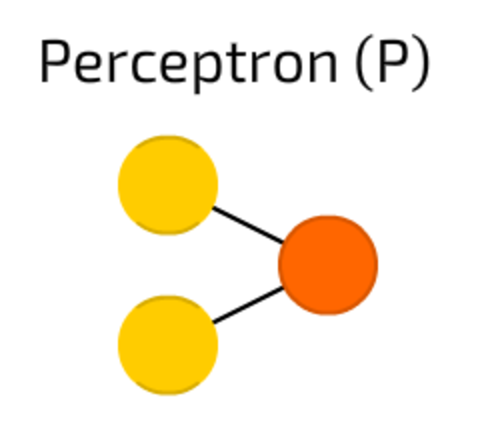
\includegraphics[trim=0 0 0 3.3cm, clip]{images/perceptron.png}}
\caption{Perceptronas.}
\label{fig:perceptron1}
\end{figure}

\begin{figure}
  \centering
\scalebox{0.7}{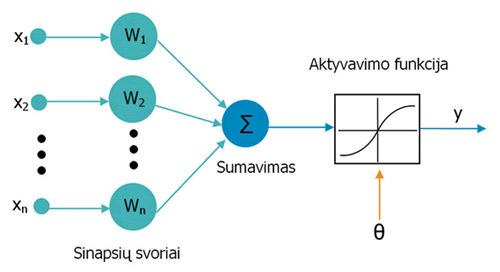
\includegraphics[trim=0 1cm 0 0, clip]{images/perceptron_pvz.png}}
\caption{Dirbtinio neurono modelis (Perceptronas).}
\label{fig:perceptron}
\end{figure}

Paveiksle pavaizduoto Perceptrono reikšmė apskaičiuojama pagal formulę
\begin{equation*}
  y = f \left(\sum_{k=1}^{n} x_k W_k \right),
\end{equation*}

čia f - aktyvavimo funkcija.

Paveiksle \ref{fig:perceptron} pavaizduoto neurono veikimo principas:
\begin{enumerate}

\item Neuronas gauna įvesties reikšmes $x_1, x_2, ... , x_n$. Kiekviena iš reikšmių turi savo perdavimo koeficientą į neuroną (svorį) $W_1, W_2, ... , W_n$.
\item  Skaičiuojama įvesties reikšmių ir atitinkamų svorių sandaugų suma ( žymima $z$).
\begin{equation*}
  z = \sum_{k=1}^{n} x_k W_k
\end{equation*}

\item  Neurono išvesties reikšmė ( žymima $a$) yra apskaičiuojama įvesties reikšmių ir atitinkamų svorių sandaugų sumai pritaikius aktyvacijos funkciją ( žymima $f$).
\begin{equation*}
  a = f(z) = f(\sum_{k=1}^{n} x_k W_k)
\end{equation*}
\end{enumerate}

\subsection{Sužadinimo signalai(angl. \textit{Bias neuron})}
Dažniausiai įvesties reikšmių yra vienetu daugiau, nei yra paduodama įvesties reikšmių. Ši įvestis yra vadinama sužadinimo signalu (angl. \textit{bias neuron}). Šio signalo reikšmė yra pastovi ir visada lygi vienetui($x_{n+1} = 1$). Taip pat yra pridedamas papildomas svoris $W_{n+1}$ jungiantis šį signalą su neuronu.\cite{Ieva2012}
Šis sužadinimo signalas padeda lengvai koreguoti neurono išvesties reikšmę, kadangi įvesties reikšmė yra vienetas, tuomet sandauga, kuri yra prisumuojama priklauso tik nuo svorio jungiančio sužadinimo signalą su neuronu. Ji yra lygi  $W_{n+1}$. Naudojant sužadinimo signalus neuroniai tinklai yra daug sparčiau apmokinami, kadangi šie signalai gali laisvai koreguoti perduodamą reikšmę į neuronus.
  \subsection{Aktyvacijos funkcijų savybės ir naudojimas(angl. \textit{Activation function})}
Neurono išvesties reikšmei apskaičiuoti naudojamų aktyvacijos funkcijų yra labai daug. Jų paskirtis yra nuspręsti ar atitinkamas neuronas, kuriam yra taikoma aktyvacijos funkcija yra reikšmingas tolimesniem skaičiavimams.

Tarkime turime neuroną, kurio $z$ yra lygus $\sum_{k=1}^{n} x_k W_k + bias$. Šios reikšmės reikšmių intervalas yra nuo $-\infty$ iki $+\infty$. Kadangi neuronai nežino reikšmių ribų, tam tikslui yra naudojamos aktyvacijos funkcijos nuspręsti ar šis neuronas turi būti sužadintas.

Aktyvacijos funkcijos negali būti tiesinės. Straipsnyje rašoma, kad tarkim turint tiesinę funkciją f(x)=cx, mes ją galime naudoti skaičiuojant kai kurių neuronų reikšmes, tačiau bendruoju atveju, kadangi neuronių tinklų tikslas yra tobulėti (t.y. mokytis). Neuroninių tinklų mokymas vyksta, naudojant gradientinio nusileidimo metodą. Šiam metodui yra reikalingos tinkluose naudojamos aktyvacijos funkcijos išvestinė. Kadangi šios tiesinės funkcijos išvestinė yra lygi konstantai, tai baudos funkcijos gradientas irgi bus lygus konstantai. Kadangi svorių atnaujinimas vyks priešinga gradiento kryptimi pagal konstantą, tai tinklas nebus apmokomas, nes funkcijos gradientas nepriklausys nuo įvesties reikšmių. \cite{Avinash2017}

Sigmoidinė netiesinė aktyvacijos funkcija. Jos funkcija $f(x)=\frac{1}{1+e^{-x}}$ ir grafikas paveiksle \ref{fig:sigmoid}.
\begin{figure}[h!]
  \centering
\scalebox{0.6}{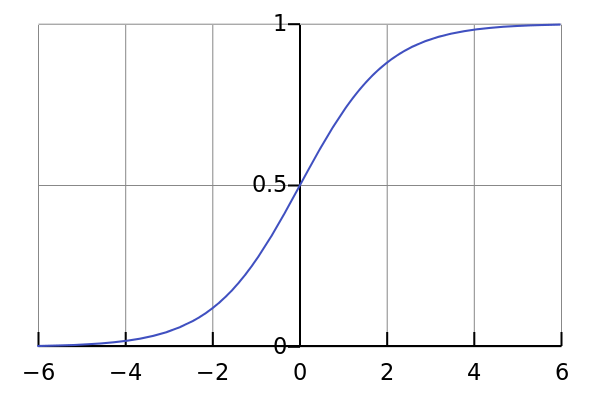
\includegraphics{images/sigmoid.png}}
\caption{Sigmoidinės funkcijos grafikas.}
\label{fig:sigmoid}
\end{figure}

Įvardinsime šios aktyvacijos funkcijos privalumus ir trūkumus. \cite{Avinash2017}
\begin{enumerate}
  \item Privalumai:
  \begin{enumerate}
    \item Netiesinė funkcija.
    \item Šios funkcijos išvestinė taip pat netiesinė funkcija.
    \item Šios funkcijos reikšmių intervalas yra nuo 0 iki 1, tai reiškia, kad funkcijos reikšmės turi rėžius, palyginus su tiesinėmis funkcijomis, kai rėžiai buvo $-\infty$ iki $+\infty$.
    \item Kai x kinta nuo -2 iki 2, tai funkcijos reikšmės yra labai stačios(mažas x pakitimas turi daug įtakos funkcijos reikšmei), o kitais atvejais funkcija gražina arba labai žemą arba labai aukštą reikšmę, kas leidžia išskirti ryškias savybes.
  \end{enumerate}
  \item Trūkumai:
  \begin{enumerate}
    \item Kai funkcijos gražinamos reikšmės yra arti 0 arba 1, tai funkcijos reikšmės labai mažai pasikeičia, kai kinta x. tai reiškia, kad gradiento reikšmė toje srityje bus maža. Tai gali sukelti gradiento išnykimą (angl. \textit{vanishing gradient}), to pasekoje tinklas mokosi labai lėtai arba išvis nesimokina, jei neįvyksta jokiu drąstinių pokyčių.
  \end{enumerate}
\end{enumerate}


Hiperbolinio tangento netiesinė aktyvacijos funkcija. Jos funkcija $f(x)=tanh(x)=\frac{2}{1+e^{-2x}}-1$ ir grafikas paveiksle \ref{fig:tanh}.

\begin{figure}[h!]
  \centering
\scalebox{0.6}{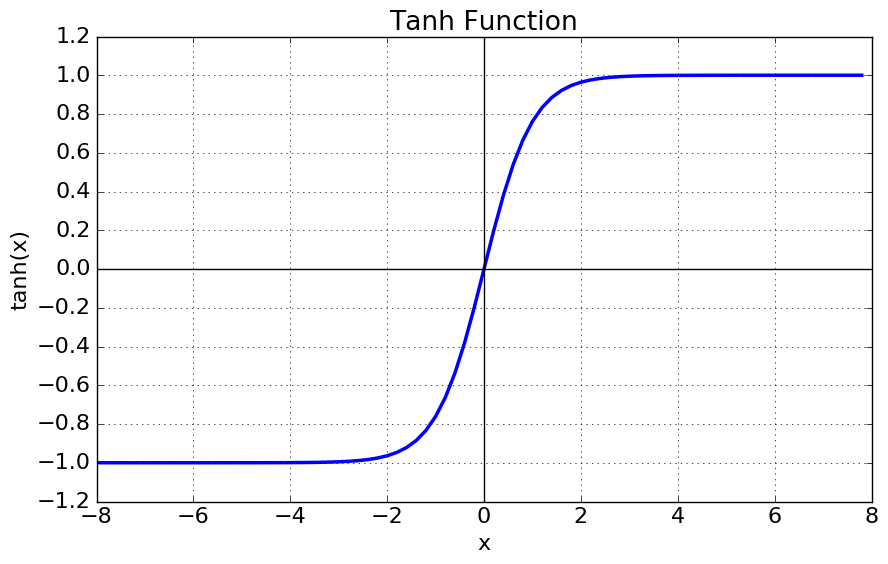
\includegraphics{images/tanhh.png}}
\caption{Hiperbolinio tangento grafikas.}
\label{fig:tanh}
\end{figure}

Įvardinsime šios aktyvavimo funkcijos privalumus ir trūkumus. \cite{Avinash2017}
\begin{enumerate}
  \item Privalumai:
    \begin{enumerate}
      \item Netiesinė funkcija.
      \item Šios funkcijos išvestinė taip pat netiesinė funkcija.
      \item Šios funkcijos reikšmių intervalas yra nuo -1 iki 1, tai reiškia, kad funkcijos reikšmės turi rėžius.
      \item Hiperbolinio tangento gradientai yra stipresni, nei sigmoidinės funkcijos(t.y. išvėstinės yra statesnės).
    \end{enumerate}
  \item Trūkumai:
    \begin{enumerate}
      \item Kaip ir sigmoidinėje funkcijoje hiperbolinis tangentas turi tą pačią nykstančio gradiento problemą.
    \end{enumerate}
\end{enumerate}


\subsection{Tiesioginio sklidimo neuroniniai tinklai(angl. \textit{Feed Forward neural networks })}

Naudojant Perceptronų sudarymo logiką, buvo pradėti kurti pradiniai tiesioginio sklidimo neuroniai tinklai. Šie tinklai yra sudaryti iš daug perceptronų, kurie yra sugrupuoti į tris sluoksnius \ref{fig:feedforfff}.
\begin{enumerate}
  \item Įvesties sluoksnis (angl. \textit{Input layer}).
  \item Paslėptasis sluoksnis (angl. \textit{Hidden layer}).
  \item Išvesties sluoksnis (angl. \textit{Output layer}).
\end{enumerate}

\textbf{Įvesties sluoksnis.} Įvesties sluoksnis sudarytas iš neuronų, kurie priima įvesties reikšmes. Šio sluoksnio neuronų reikšmės yra tokios pat kaip ir įvesties reikšmės. \cite{Sibanjan2017}

\textbf{Išvesties sluoksnis.} Išvesties sluoksnis yra paskutinis šio neuroninio tinklo sluoksnis, kuris vartotojui gražina tinklo apskaičiuotas reikšmes. \cite{Sibanjan2017}

\textbf{Paslėptasis sluoksnis.} Paslėptasis sluoksnis yra išdėstytas taip, kad į jį įeinantys neuronai yra įvesties sluoksnio neuronai, o šio paslėptojo sluoksnio neuronai įeina į išvesties sluoksnio neuronus. Tai yra tarpinis sluoksnis tarp įvesties ir išvesties sluoksnių. \cite{Sibanjan2017}

\begin{figure}[h!]
  \centering
\scalebox{0.8}{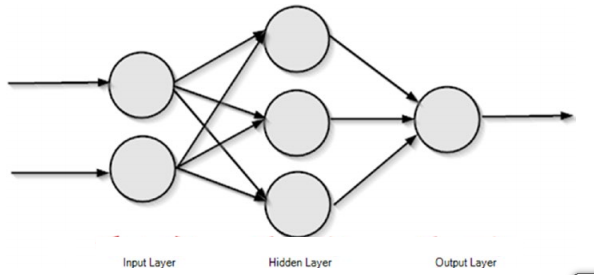
\includegraphics{images/ffnettt.png}}
\caption{Tiesioginio sklidimo neuroninis tinklas.}
\label{fig:feedforfff}
\end{figure}

Paveiksle \ref{fig:feedforfff} galima pastebėti, kad
\begin{enumerate}
  \item Du gretimi esantys sluoksniai yra pilnai sujungti svoriais.
  \item Reikšmių apskaičiavimas vyksta pradedant įvesties sluoksniu, toliau reikšmes perduodant paslėptajam sluoksniui ir pabaigoje iš paslėptojo sluoksnio reikšmes perduodant išvesties sluoksniui.
  \item Tarp įvesties ir išvesties sluoksnių yra vienas paslėptasis sluoksnis.
\end{enumerate}


\subsection{Daugiasluoksniai tiesioginio sklidimo neuroniniai tinklai(angl. \textit{Deep Feed Forward neural networks})}

Turintys daugiau nei vieną paslėptajį sluoksnį, tiesioginio sklidimo neuroniniai tinklai yra vadinami daugiasluoksniais. Šio tinklo veikimo principas yra toks pat, kaip ir paprastojo tiesioginio neuroninio tinklo su vienu paslėptuoju sluoksniu. Šių tinklų privalumas yra tas, kad kiekvienas paslėptasis sluoksnis nustato tam tikras įvesties duomenų charakteristikas. Pavyzdžiui \cite{Deividas2018} darbe rašoma, kad atliekant šį tinklą apmokant atpažinti ranka rašytinius skaičius, tinklo paslėptieji sluoksniai nusako tam tikras skačiaus charakteristikas, pavyzdžiui vienas sluoksnis gali nusakyti ar skaičiuje yra apskritimas, tai jei sluoksnis atranda apskritimą tame skaičiuoje, tai tinklo gražinamos reikšmės gali būti 0, 6, 8 arba 9, kadangi šiuose skaičiuose yra apskritimas.

Norint žinoti kiek sluoksnių yra šiuose neuroniniuose tinkluose, skaičiavimams atlikti yra įvedamas žymėjimas L, kuris reiškia kiek sluoksnių šitame neuroniniame tinkle yra, o žymėjimas l reiškia kuriame sluoksnyje dabar atliekame skaičiavimus.

\begin{figure}[h!]
  \centering
\scalebox{0.4}{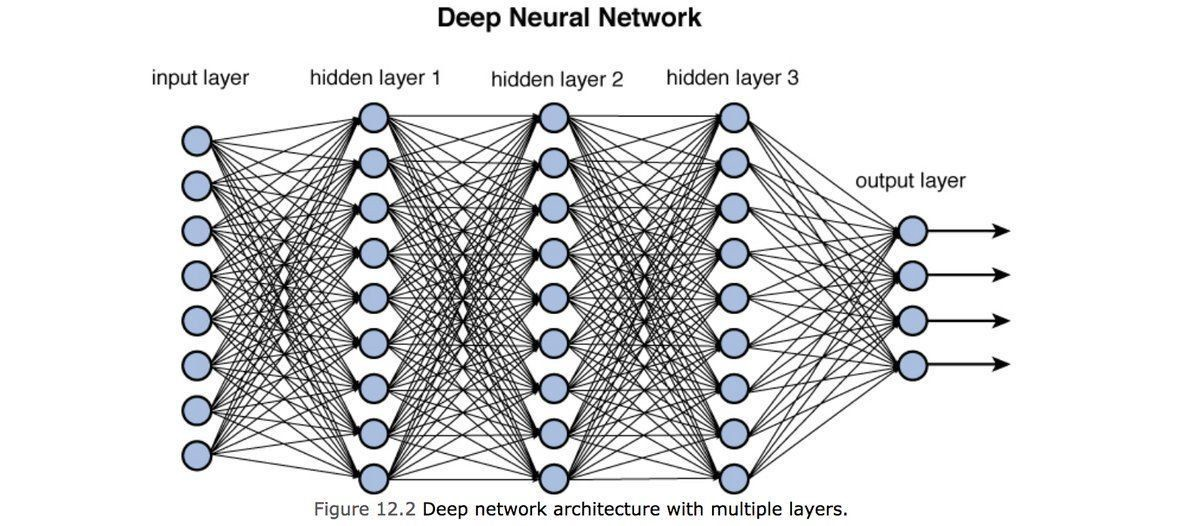
\includegraphics[trim=0 1cm 0 1.8cm, clip]{images/deepff.jpeg}}
\caption{Daugiasluoksnis tiesioginio sklidimo neuroninis tinklas.}
\label{fig:deepnn}
\end{figure}

Šio tinklo bet kurio neurono skaičiavimo formulė.

\begin{equation*}
  a_k^l = f(\sum_{n=1}^{s_{l-1}} a_n^{l-1}W_{nk}^{l-1} + bias),
\end{equation*}
čia $s_l$ - nurodo kiek l-ajame sluoksnyje yra neuronų, $a_k^l$ - nurodo k-ąjį neuroną l-ajame sluoksnyje, o $W_{nk}^{l-1}$ - nurodo svorį jungiantį (l-1)-ojo sluoksnio n-ajį neuroną su l-ojo sluoksnio k-uoju neuronu.

\subsection{Rekurentiniai neuroniniai tinklai(angl. \textit{Recurrent Neural Network})}

Rekurentiniai neuroniai tinklai implementuoja naujo tipo ląsteles, vadinamas rekurentinėmis ląstelėmis. Pirmasis šio tinklo prototipas buvo sukurtas, taip kad kiekviena paslėpta tinklo ląstelė kaip įvestis pasiimdavo tos pačios ląstelės išvesties reikšmes kelių žingsnių.

Yra daug šio tinklo variacijų, pavyzdžiui kaip įvestis perduoti tinklo būsenas, kintamųjų užtempimas ir panašiai, tačiau įdėja išlieka ta pati. Šis tinklas dažniausiai yra naudojamas, kai yra svarbus kontekstas (t.y. kai sprendimai priklauso nuo to kas vyko praeityje), pavyzdžiui sudarant tekstus, nauji teksto sakiniai yra prognozuojami, pagal tai kokie sakiniai jau yra prieš tai parašyti.


\subsection{ LSTM tipo rekurentiniai neuroniniai tinklai(angl. \textit{LSTM Recurrent Neural Network})}

LSTM - Ilgalaikė/trumpalaikė atmintis. Šio tipo rekurentiniai tinklai implementuoja atminties ląstelę, kuri gali apdoroti duomenis, kai paduodami duomenys turi tam tikrus laiko tarpus, kada jie yra paduodami. Šie tinklai gali prognozuoti tekstą pagal pavyzdžiui 10 prieš tai einančių žodžių. Taip pat šie tinklai gali prognozuoti vaizdo kadrą, pagal tai kas vyko keliais kadrais ankščiau. \cite{Christopher2015}

Atminties ląstelės yra sudarytos iš kelių elementų vadinamų vartais(angl. \textit{gates}), kurie kontroliuoja kaip informacija yra prisimenama ir pamirštama.

Mūsų darbe naudojamo tinklo vartų ląstelių yra keturios:
\begin{enumerate}
  \item Pamiršimo vartai (angl. \textit{forget gate}).
  \item Įvesties vartai (angl. \textit{input gate}).
  \item Įvesties moduliacijos vartai (angl. \textit{input modulation gate}).
  \item Išvesties vartai (angl. \textit{output gate}).
\end{enumerate}

Kiekviena iš keturių tinklo ląstelių yra sudaryta iš daugiasluoksnių tiesioginių neuroninių tinklų. Kiekviena iš ląstelių atlieka savo vaidmenį šiame tinkle.

\begin{enumerate}
  \item Pamiršimo ląstelė nurodo, kuri perduodama informacija turi būti pamirštama, nereikšminga.
  \item Įvesties ląstelė kontroliuoja kiek naujos informacijos iš įvesties reikšmių reikia pridėti prie jau esamos informacijos.
  \item Įvesties moduliacijos ląstelė papildomai pakoreguoja kiek naujas informacijos reikia pridėti prie jau esamos informacijos.
  \item Išvesties ląstelė nurodo, kuri informacija yra svarbi ir kiek jos turi būti perduodama tolimesniems skaičiavimam.
\end{enumerate}

Šių visų tinklų perduodama informacija sąveikauja tarpusavyje. \ref{fig:lstmveikimas}

\begin{figure}[h!]
  \centering
\scalebox{0.4}{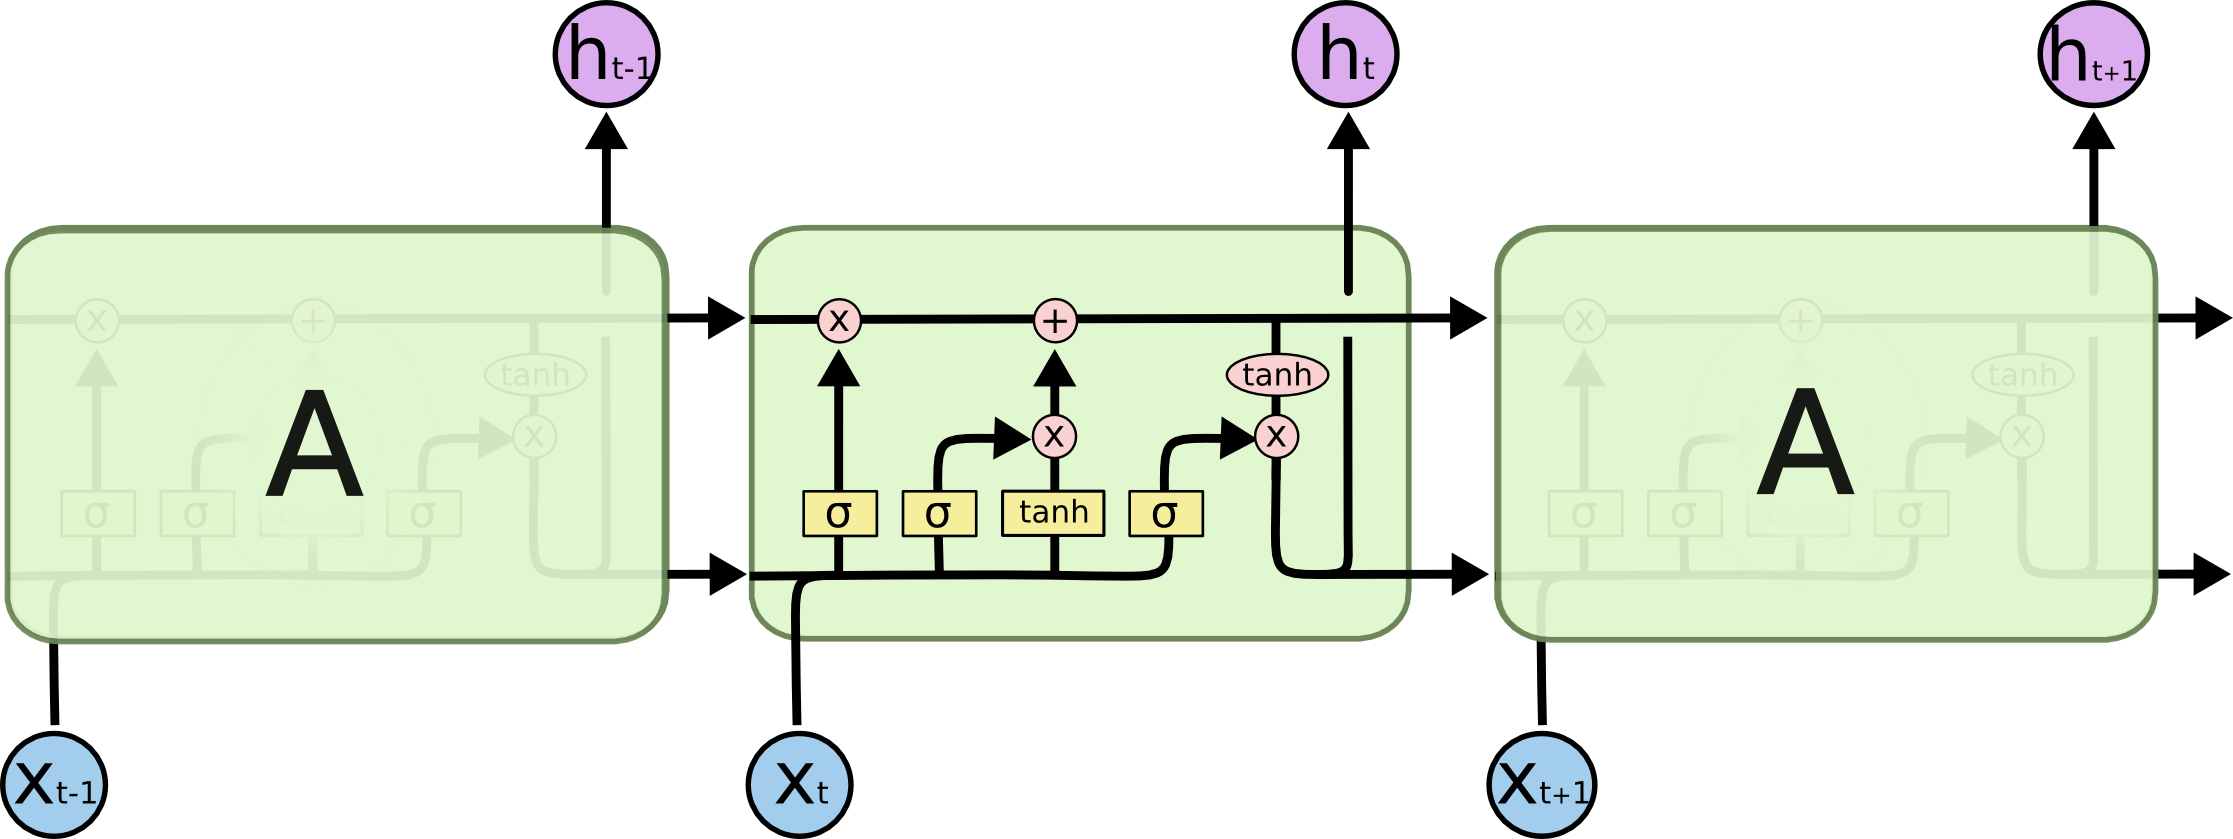
\includegraphics{images/LSTMveikimas.png}}
\caption{LSTM tinklo sandara.}
\label{fig:lstmveikimas}
\end{figure}

Pagrindinė šio tinklo veikimo esmė yra atmintis, kuri yra perduodama kaip būsena prognozuojant naujas tinklo išvesties reikšmes.

\begin{figure}[h!]
  \centering
\scalebox{0.6}{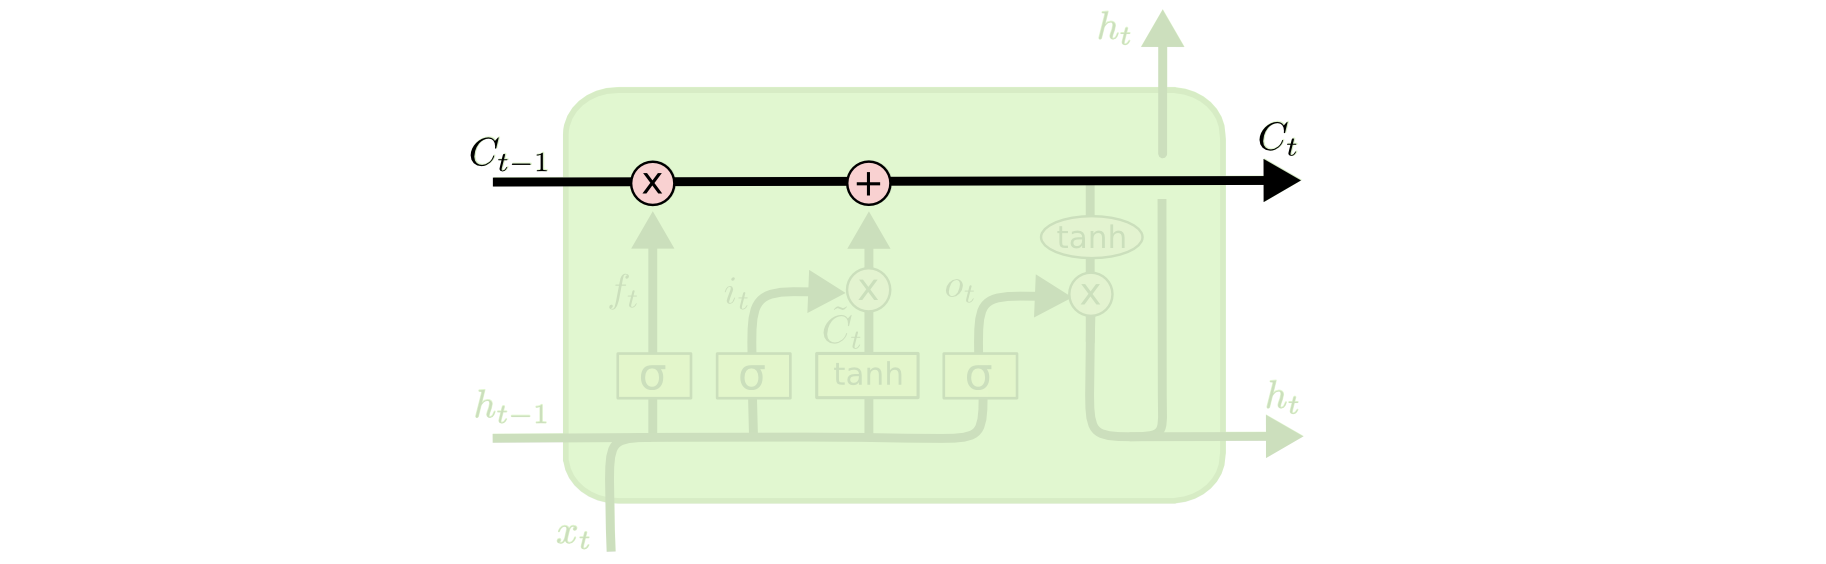
\includegraphics{images/LSTMcore.png}}
\caption{LSTM tinklo atmintis.}
\label{fig:lstmcore}
\end{figure}

LSTM tinklai turi galimybę ištrinti arba įrašyti informaciją į atmintį. Kuri informacija yra perduodama arba pamirštama yra kontroliuojama ląstelių, kurios yra neuroniniai tinklai su individualiomis charakteristikomis.\cite{Christopher2015}

Rekurentinis neuroninis tinklas turi tris neuroninius tinklus, kurie naudoja sigmoidinę aktyvacijos funkciją ir vieną tinklą, kuris naudoja hiperbolinio tangento aktyvacijos funkciją.

LSTM veikimo principas \cite{Christopher2015}
\begin{enumerate}
  \item Pirmiausia nustatome, kurią informaciją turime pamiršti. Šį sprendimą daro pamiršimo ląstelė. Ji pagal tinklo būseną ir įvesties reikšmes nustato, kurią informaciją reikia visiškai pamirši, o kurią reikia perduoti. \ref{fig:lstmforget}
  \begin{figure}[h!]
    \centering
  \scalebox{0.6}{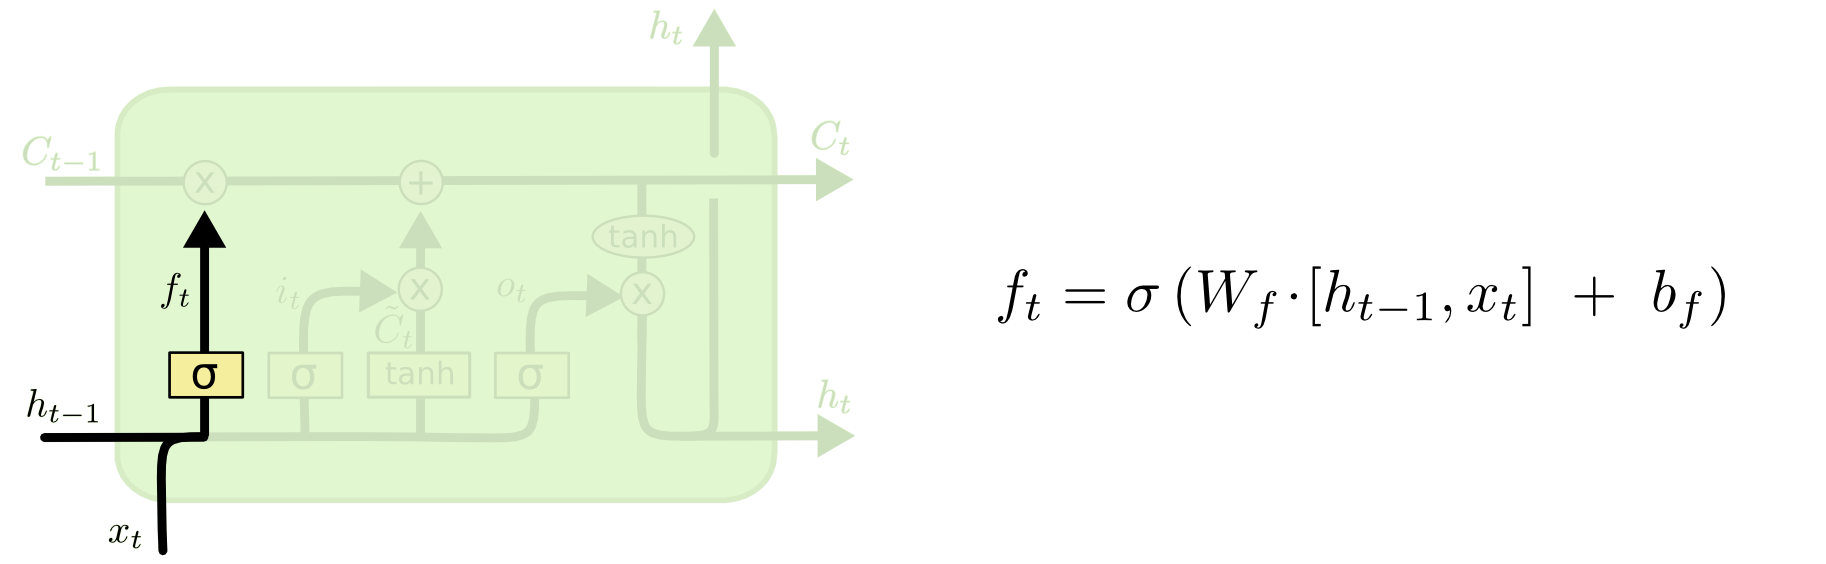
\includegraphics[trim=0 0 11cm 0, clip]{images/LSTMforget.png}}
  \caption{LSTM tinklo pamiršimo ląstelė.}
  \label{fig:lstmforget}
  \end{figure}
  \item Sekantis žingsnis yra nustatyti kurią informaciją įrašysime į atmintį. Šį sprendimą daro įvesties ir įvesties moduliacijos ląstelės. Įvesties ląstele nustatome, kurią informaciją mes pridėsime, o įvesties moduliacijos ląstele nustatome kokia ta informacija bus. \ref{fig:lstminput}
\begin{figure}[h!]
  \centering
\scalebox{0.6}{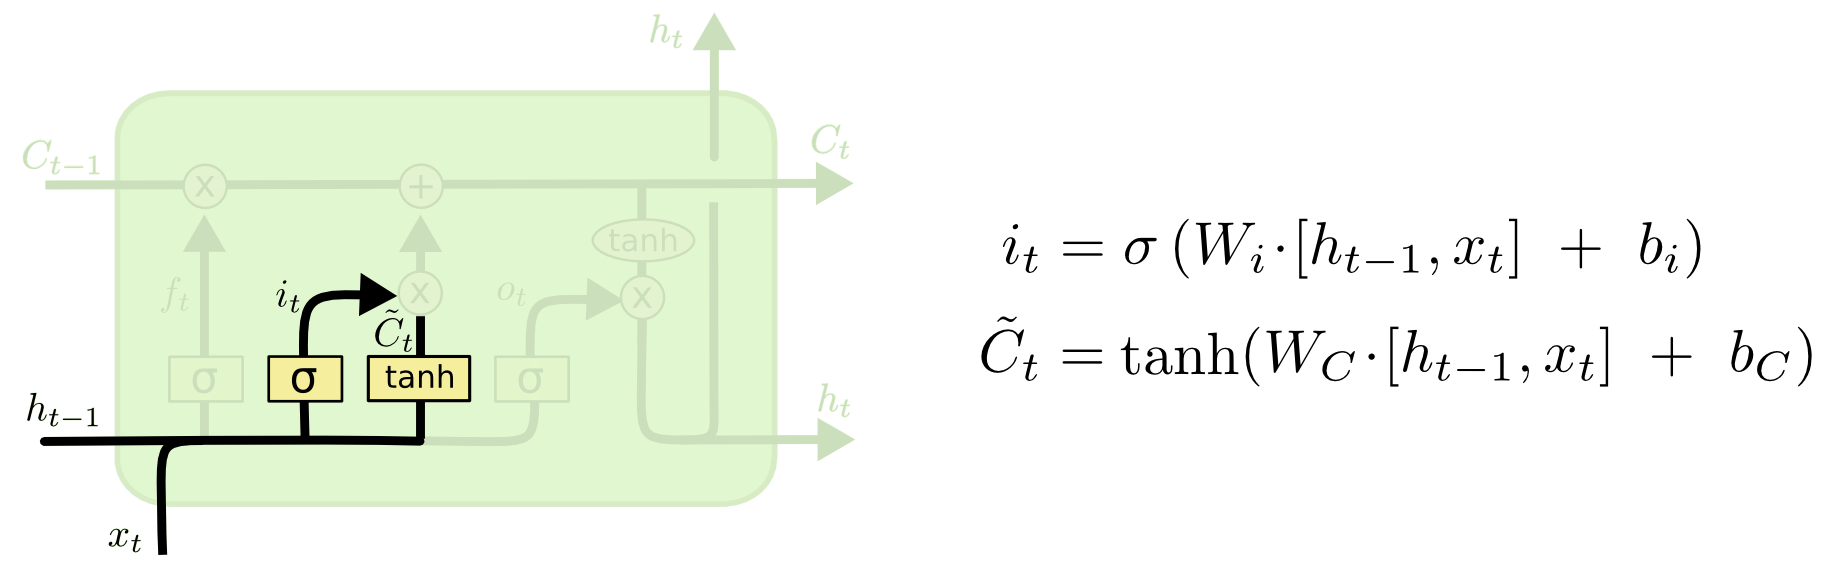
\includegraphics[trim=0 0 11cm 0, clip]{images/LSTMinput.png}}
\caption{LSTM tinklo įvesties ląstelės.}
\label{fig:lstminput}
\end{figure}
\item Toliau atnaujinsime tinklo atmintį. Iš pradžių padauginame atmintį iš pamiršimo ląstelės, kad pamirštume informaciją, kurią nustatėme, kad reikia pamiršti. o toliau pridėsime informaciją, kurią nustatė įvesties ir įvesties moduliacijos ląstelės, kad reikia pridėti.\ref{fig:lstmnewc}
\begin{figure}[h!]
  \centering
\scalebox{0.6}{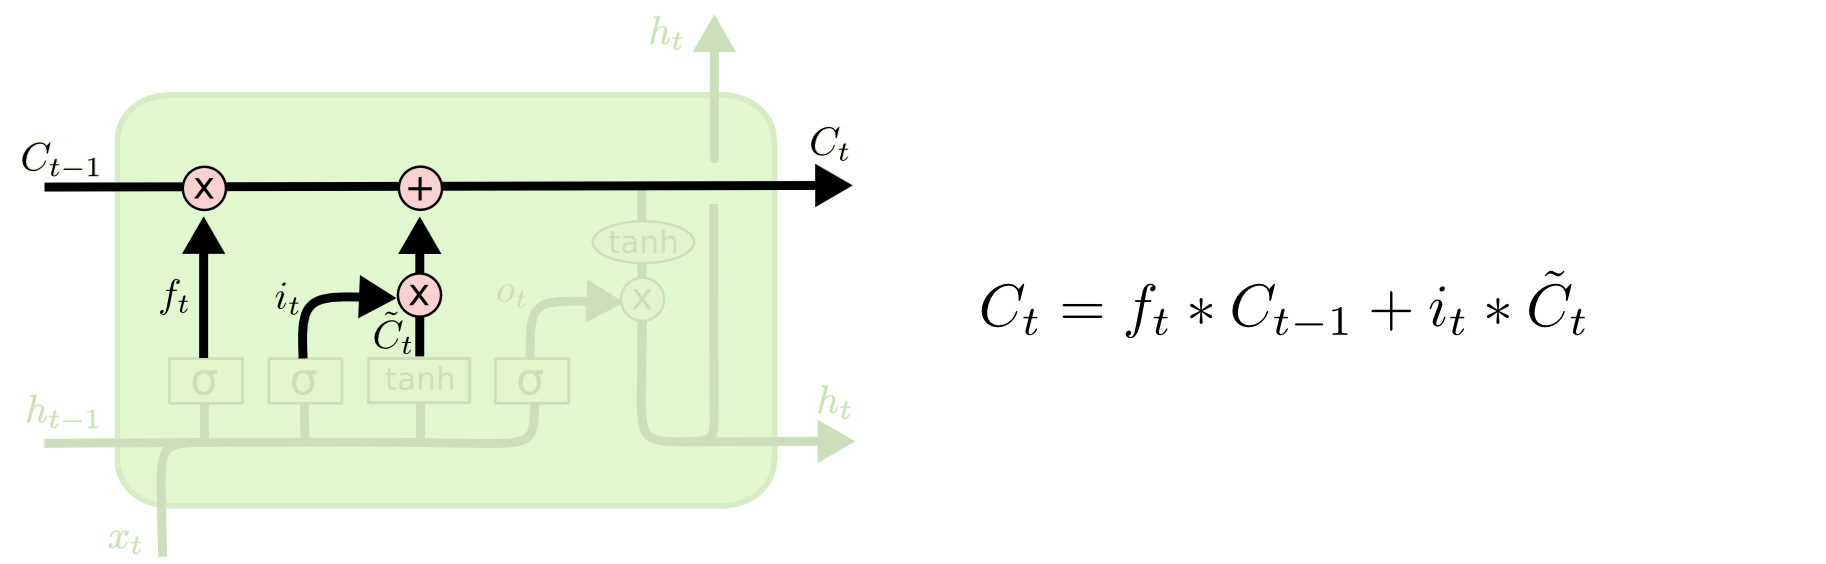
\includegraphics[trim=0 0 11cm 0, clip]{images/LSTMnewc.png}}
\caption{LSTM tinklo naujos atminties skaičiavimas.}
\label{fig:lstmnewc}
\end{figure}
\item Galiausiai nustatome kokią tinklo reikšmę išvesime. Ši reikšmė priklausys nuo naujos atminties ir išvesties ląstelės. Išvesties ląstelė nustato kurias reikšmes reikia perduoti, o atminčiai yra pritaikoma hiperbolinio tangento funkcija. Sudauginus atmintį ir išvesties ląstelę, gauname kurią informaciją išvesime.\ref{fig:lstmoutput}
\begin{figure}[h!]
  \centering
\scalebox{0.6}{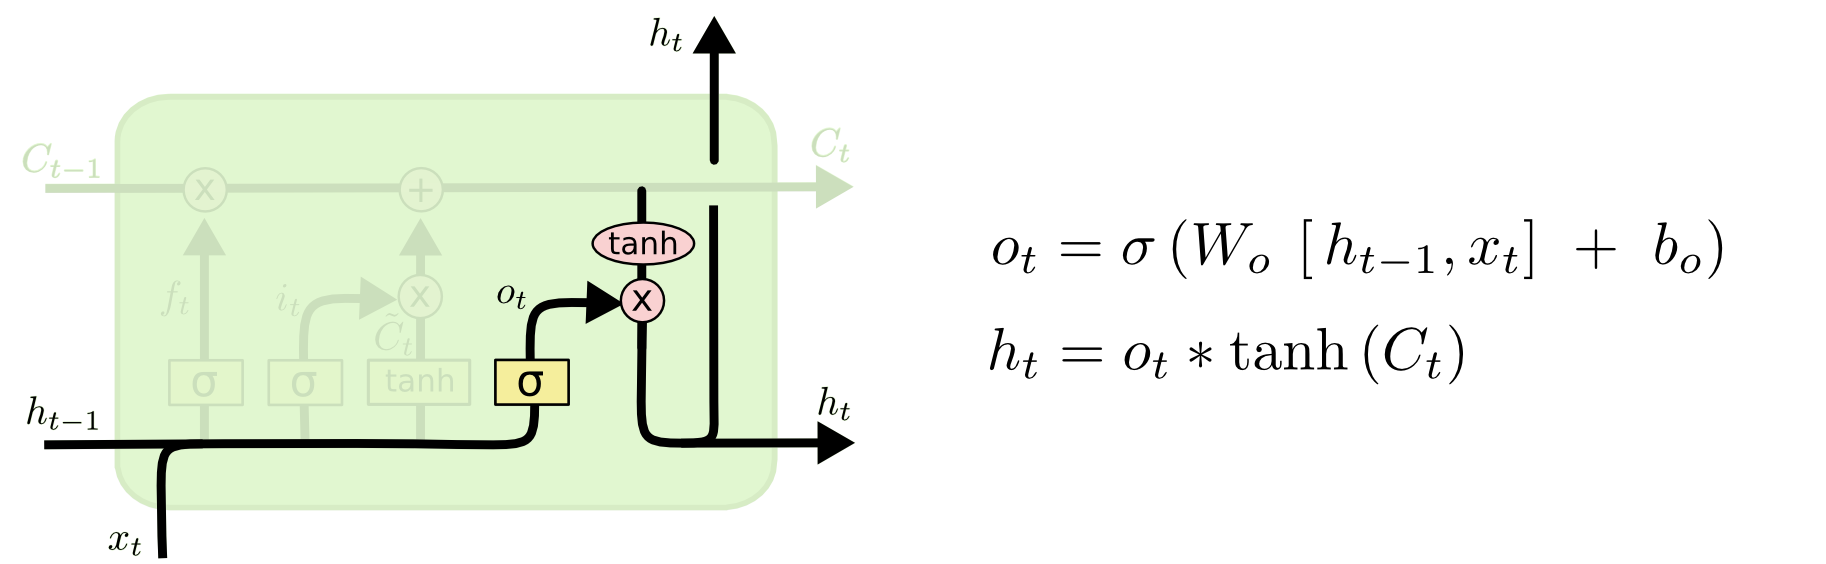
\includegraphics[trim=0 0 11cm 0, clip]{images/LSTMoutput.png}}
\caption{LSTM tinklo naujos atminties skaičiavimas.}
\label{fig:lstmoutput}
\end{figure}
\end{enumerate}

Tačiau mano kuriamame tinkle išvesties reikšmė dar nebus galutinė. Šiuo atveju naudosiu softmax funkciją, kuri išvesties reikšmes normalizuos į tikimybinį pasiskirstymą. Ši funkcija yra naudojama, kadangi išvesties reikšmių intervalas yra nuo -1 iki 1 ir šių reikšmių suma gali būti nelygi vienetui, tačiau pritaikius šią funkciją išvesties reikšmių intervalas yra nuo 0 iki 1 ir išvesties reikšmių suma yra lygi vienetui, tam kad būtų galima patogiau suprasti tinklo išvestį.

Rekurentinio tinklo apmokymas vyksta klaidos sklidimo atgal metodu(angl. \textit{back propogation}).

\textbf{Tinklo apmokymo principas}

Tinklo apmokymas grindžiamas minimizuojant tinklo baudos funkcijos išvestinę pagal visus tinkle esančius svorius.
    \begin{equation*}
      \frac{\partial E}{\partial W_{ij}}
    \end{equation*}
Naudojant šią išvestinę tinklo apmokymas vykdomas atnaujinant visus tinklo svorius.
    \begin{equation*}
      W_{ij} = W_{ij} + \frac{\partial E}{\partial W_{ij}}
    \end{equation*}
Tačiau toks tinklo apmokymo būdas nėra veiksmingas, nes tinklas apsimokys atpažinti naujas reikšmes labai greitai, tačiau problema yra ta, kad labai lengvai pamirš ką jau išmoko praeityje, todėl yra naudojami $\alpha$ ir $\eta$ koeficientai. Gaunama nauja formulė.
\begin{equation*}
  \Delta W_{ij} =-\eta\frac{\partial E}{\partial W_{ij}}+\alpha \Delta W_{ij} \\
    W_{ij} = W_{ij} + \Delta W_{ij}
\end{equation*}
$\alpha$ ir $\eta$ kintamieji nurodo tinklo apmokymo inerciją ir greitį. \cite{Deividas2018} darbe lyginamos tinklo apmokymo paklaidos keičiant šių parametrų reikšmes. Parinkus optimalius parametrus tinklo svoriai daug greičiau konverguoja į norimus svorius, kas leidžia tinklui greičiau apsimokinti. Parinkus labai mažas apmokymo greičio reikšmes tinklas gali labai užtrukti, kol jis apsimokins, o parinkus labai dideles reikšmes tinklas labai greitai išmoks atpažinti naujas reikšmes, tačiau pamiršdamas senas.


\subsection{ Informatikos apžvalga}



% Reukurentinio neuroninio tinklo apmokymas vyksta į tinklą paduodant tam tikrus rinkinius duomenų. Tie rinkiniai sudaryti iš įvesties reikšmių ir reikšmių, kurias tikimasi gauti iš tinklo. Iš pradžių duomenys yra praleidžiami pro tinklą (angl. \textit{Feed forward}) ir poto atliekamas baudos funkcijos paklaidos mažinimas anti-gradientinio nusileidimo metodu (angl. \textit{Back Propogation}).
%
%
%
%
%
%
%
%
%
%
%
%
%
%
% Patys pirmieji neuroninio tinklo modeliai buvo sukurti Tiesioginio sklidimo (angl. \textit{Feed forward}) neuroniniai tinklai.
%
% \cite{Ieva2012}
%
%
% %padaryti feedforward vieno apskaiciavima
% Šiuo būdu realizuoto neurononio tinklo schema pavaizduota (). Čia


% Dirbtinis intelektas
%
%
% neuroniai tinklai, ju tipai
%
%
% Neuroninių tinklų yra daug tipų, pagal
%
%
%
% lstm neuroninis tinklas
%
% taikymas language Modelling
%
%
% Dirbtinis intelektas
